% DISPLAYING DATA: HISTOGRAMS \& BOX PLOTS - WORKSHEET 0
\documentclass[12pt, letterpaper, fleqn]{article}

% ----------------------------------------------------------
% PACKAGES
% ----------------------------------------------------------
\usepackage{graphicx}
\usepackage{xcolor}
\usepackage[most]{tcolorbox}
\usepackage{amsmath, amssymb}
\usepackage{fancyhdr}
\usepackage[utf8]{inputenc}
\usepackage[T1]{fontenc}
\usepackage{enumitem}
\usepackage{geometry}
\usepackage{tikz}
\usepackage{needspace}
\usepackage{multicol}

\usetikzlibrary{arrows.meta, calc}

% ----------------------------------------------------------
% PAGE SETUP
% ----------------------------------------------------------
\usepackage{times}
\geometry{letterpaper, top=1.25in, bottom=1.25in, marginpar=0.5in}

% ----------------------------------------------------------
% HEADER / FOOTER
% ----------------------------------------------------------
\newcommand{\logowidth}{3cm}
\setlength{\headheight}{20pt}
\setlength{\footskip}{40pt}

\pagestyle{fancy}
\fancyhf{}
\fancyhead[C]{\small\bfseries Displaying Data: Histograms \& Box Plots}
\fancyfoot[L]{\raisebox{2pt}{
\includegraphics[width=\logowidth]{kss.png}}}
\fancyfoot[C]{\thepage}
\fancyfoot[R]{6.23.0}

\renewcommand{\footrulewidth}{0.2pt}

% ----------------------------------------------------------
% HELPER MACROS
% ----------------------------------------------------------
\newcommand{\blank}{\underline{\hspace{2.2cm}}}
\newcommand{\blanklong}{\underline{\hspace{6.5cm}}}
\newcommand{\blankshorter}{\underline{\hspace{1.5cm}}}

% ----------------------------------------------------------
% DOCUMENT
% ----------------------------------------------------------
\begin{document}


\textbf{Name:} \underline{\hspace{5cm}}
\hfill
\textbf{Date:} \underline{\hspace{3cm}}\\

% ==========================================================
% SECTION 1: HISTOGRAMS AND BOX-AND-WHISKER PLOTS
% ==========================================================
\begin{tcolorbox}[colback=black!10]
    \large\textcolor{black}{\textbf{Histograms and Box-and-Whisker Plots (Foundation)}}
\end{tcolorbox}

\vspace{1mm}

\noindent
1. \textbf{Histogram:} A continuous distribution summary where individual data entries are sorted into uniform, non-overlapping intervals (\textbf{bins}). Heights represent the direct frequency count of observations inside that range.
2. \textbf{Box Plot:} A visual map dividing data into numerical quarters ($25\%$ intervals) via a five-point benchmark array:
\begin{itemize}[noitemsep, leftmargin=0.5cm]
    \item \textbf{Minimum / Maximum:} The lowest and highest boundaries of non-outlier entries.
    \item \textbf{Median ($Q_2$):} The exact midpoint separating the upper and lower halves of data.
    \item \textbf{Lower Quartile ($Q_1$):} The center value of the bottom half ($25^{\text{th}}$ percentile).
    \item \textbf{Upper Quartile ($Q_3$):} The center value of the top half ($75^{\text{th}}$ percentile).
\end{itemize}
3. \textbf{Interquartile Range (IQR):} Defined mathematically as $Q_3 - Q_1$, tracking the width of the main box containing the interior $50\%$ of the observations.

\vspace{2mm}

% --- FIXED GEOMETRIC VISUAL MODELS PANEL ---
\begin{center}
\begin{tikzpicture}[scale=0.8]
    % --- BOX PLOT SUITE (TOP) ---
    % Axis Line
    \draw[thick,->] (0,0) -- (11,0);
    \foreach \x in {0,2,4,6,8,10} \draw (\x, 0.1) -- (\x, -0.1) node[below, scale=0.75] {\x};
    
    % Box Construction
    \draw[thick] (2, 0.6) -- (4, 0.6); 
    \draw[thick] (9, 0.6) -- (10, 0.6); 
    \draw[thick, fill=black!5] (4, 0.2) rectangle (9, 1.0); 
    \draw[ultra thick, red] (6, 0.2) -- (6, 1.0); 
    
    % End Cap Lines
    \draw[thick] (2, 0.4) -- (2, 0.8); 
    \draw[thick] (10, 0.4) -- (10, 0.8); 
    
    % Typography Annotations
    \node[anchor=south, scale=0.7] at (2, 0.8) {Min (2)};
    \node[anchor=south, scale=0.7] at (4, 1.0) {$Q_1$ (4)};
    \node[anchor=south, scale=0.7, red!80!black] at (6, 1.0) {Med (6)};
    \node[anchor=south, scale=0.7] at (9, 1.0) {$Q_3$ (9)};
    \node[anchor=south, scale=0.7] at (10, 0.8) {Max (10)};
    
    \draw[latex-latex, thick, blue] (4, -0.6) -- (9, -0.6);
    \node[blue, fill=white, scale=0.7] at (6.5, -0.6) {$\text{IQR} = Q_3 - Q_1 = 5$};
    \node[scale=0.8, font=\bfseries] at (5, 1.7) {Box Plot Components};
\end{tikzpicture}

\vspace{1cm}

\begin{tikzpicture}[scale=0.8]
    % --- HISTOGRAM SUITE (BOTTOM) ---
    \draw[thick, <->] (0,2.5) node[left, scale=0.7] {Freq} -- (0,0) -- (10,0) node[below, scale=0.7] {Bins};
    \foreach \y in {1,2} \draw (0.1, \y) -- (-0.1, \y) node[left, scale=0.7] {\y};
    
    % Bar Groups
    \draw[fill=black!15] (1,0) rectangle (3, 0.8);
    \draw[fill=black!15] (3,0) rectangle (5, 2.0);
    \draw[fill=black!15] (5,0) rectangle (7, 1.4);
    \draw[fill=black!15] (7,0) rectangle (9, 0.8);
    
    \node[below, scale=0.7] at (2,0) {0--5};
    \node[below, scale=0.7] at (4,0) {6--10};
    \node[below, scale=0.7] at (6,0) {11--15};
    \node[below, scale=0.7] at (8,0) {16--20};
    
    \node[scale=0.8, font=\bfseries] at (5, 2.6) {Histogram Bin Formatting};
\end{tikzpicture}
\end{center}

\vspace{1mm}

\begin{tcolorbox}[colback=white, colframe=black!25, boxrule=0.6pt, arc=4mm, left=6mm, right=6mm, top=4mm, bottom=4mm]
\textbf{Worked Example:}
Find the 5-number summary of the ordered set: $2, 4, 5, 6, 8, 9, 10$.\\
\textbf{Solution:}\\
- Median ($Q_2$) is the center value: $6$.\\
- Lower sub-block is $\{2, 4, 5\}$, revealing a center lower quartile $Q_1 = 4$.\\
- Upper sub-block is $\{8, 9, 10\}$, revealing a center upper quartile $Q_3 = 9$.\\
- Min $= 2$, Max $= 10$. $\text{IQR} = Q_3 - Q_1 = 9 - 4 = 5$.
\end{tcolorbox}

\newpage

% ==========================================================
% DEEPER THINKING PROBLEM 1
% ==========================================================
\begin{tcolorbox}[colback=white, colframe=black, boxrule=1pt, arc=4mm, left=6mm, right=6mm, top=5mm, bottom=5mm]
\textbf{Deeper Thinking Problem 1: Constructing the 5-Number Summary}

\medskip

\noindent
\textbf{a)} A list of test scores is: 65, 70, 75, 80, 85, 90, 95, 100. Find the 5-number summary (Min, $Q_1$, Median, $Q_3$, Max) and calculate the IQR. Explain your process.

\vspace{3.5cm}

\noindent
\textbf{b)} Describe the difference between a bar chart and a histogram. Can you find the exact values of the individual data points from a histogram? Explain.

\vspace{3cm}
\end{tcolorbox}

\vspace{0.2cm}

% ==========================================================
% DEEPER THINKING PROBLEM 2
% ==========================================================
\begin{tcolorbox}[colback=white, colframe=black, boxrule=1pt, arc=4mm, left=6mm, right=6mm, top=5mm, bottom=5mm]
\textbf{Deeper Thinking Problem 2: Box Plot Interpretations}

\medskip

\noindent
\textbf{a)} A box plot has a very long right whisker and a short left whisker. What does this tell you about the shape and spread of the data distribution?

\vspace{3.5cm}

\noindent
\textbf{b)} If a data set has 12 values, how many values fall within the box of its box plot? Explain.

\vspace{3cm}
\end{tcolorbox}

\newpage

% ==========================================================
% DEEPER THINKING PROBLEM 3
% ==========================================================
\begin{tcolorbox}[colback=white, colframe=black, boxrule=1pt, arc=4mm, left=6mm, right=6mm, top=5mm, bottom=5mm]
\textbf{Deeper Thinking Problem 3: Mathematical Shifts in Visual Summaries}

\medskip

\noindent
\textbf{a)} Explain why a school counselor might prefer to use a box plot rather than a histogram to compare the exam scores of two different grade levels.

\vspace{5cm}

\noindent
\textbf{b)} A researcher notices that a dataset has an outlier that is extremely high. Explain how this outlier will affect the box plot's whiskers and the box itself. Will it change the IQR?

\vspace{5cm}

\noindent
\textbf{c)} New Instruction Prompt: If every individual data point in an observed dataset is doubled, what happens to the total absolute range, the positions of $Q_1$ and $Q_3$, and the final calculated IQR? Show a structural algebraic proof or step example to verify.

\vspace{5cm}
\end{tcolorbox}

\vspace{3mm}

% ==========================================================
% DEEPER THINKING PROBLEM 4
% ==========================================================
\begin{tcolorbox}[colback=white, colframe=black, boxrule=1pt, arc=4mm, left=6mm, right=6mm, top=5mm, bottom=5mm]
\textbf{Deeper Thinking Problem 4: Analyzing Outliers via IQR}

\medskip

\noindent
\textbf{a)} A standard math rule defines an outlier as any value that is more than $1.5 \times \text{IQR}$ below $Q_1$ or above $Q_3$. If a dataset has $Q_1 = 20$ and $Q_3 = 30$, what is the IQR? What are the boundaries for a value to be considered an outlier?

\vspace{5cm}

\noindent
\textbf{b)} If a student scored $5$ points in the dataset described above, is their score an outlier according to the formula? Show your work.

\vspace{5cm}

\noindent
\textbf{c)} Explain why the IQR is considered a more stable measure of spread than the range when outliers are present.

\vspace{5cm}
\end{tcolorbox}


\end{document}
\end{document}
